\section{Nivel 0 --- Protección}

\begin{frame}{Nivel 0}
  \begin{itemize}
    \item Capa de protección más baja, pero con mayor jerarquía.
    \item Salvaguarda la integridad de la grúa, la carga y el personal.
    \item Autoridad para sobrescribir cualquier comando del Nivel 1, cortando energía y aplicando frenos.
    \item Supervisa la planta de forma \textbf{permanente} (redundancia de sensores).
  \end{itemize}
\end{frame}

\begin{frame}{Autómata de seguridad: frenado selectivo}
  \begin{columns}[T]
    \begin{column}{0.45\textwidth}
      \begin{itemize}
        \item Estado nominal \texttt{SISTEMA\_OK} (ambos frenos abiertos).
        \item \textbf{Frenado selectivo}: sólo se detiene el \textbf{eje afectado}.
          \begin{itemize}
            \item Falla izaje $\Rightarrow$ frena izaje, carro libre.
            \item Falla carro $\Rightarrow$ frena carro, izaje libre.
            \item Emergencia manual $\Rightarrow$ ambos.
          \end{itemize}
        \item Rearme manual $\to$ \texttt{RECUPERACION}.
      \end{itemize}
    \end{column}
    \begin{column}{0.55\textwidth}
      \centering
      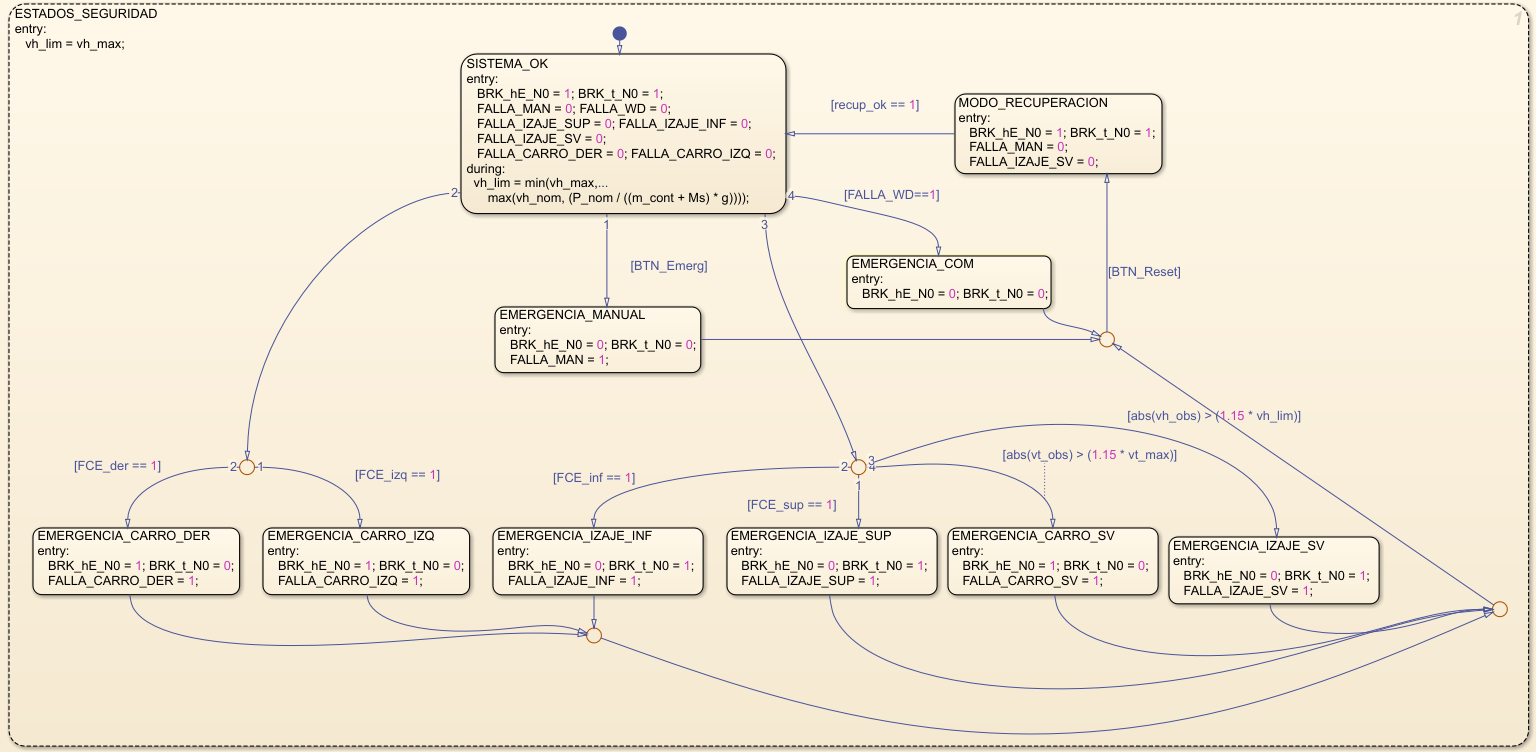
\includegraphics[width=\linewidth]{nivel_0/estados_seguridad.png}
    \end{column}
  \end{columns}
\end{frame}

\begin{frame}{Monitor de comunicaciones}
  \begin{columns}[T]
    \begin{column}{0.4\textwidth}
      \begin{itemize}
        \item Persigue el \textbf{heartbeat} del supervisor.
        \item Si el contador supera el límite seguro $FALLA_{WD}$.
        \item Dispara la parada de emergencia.
      \end{itemize}
    \end{column}
    \begin{column}{0.6\textwidth}
      \centering
      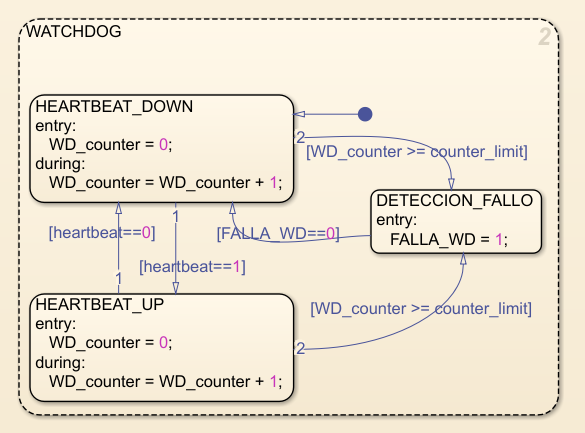
\includegraphics[width=\linewidth]{nivel_0/watchdog.png}
    \end{column}
  \end{columns}
\end{frame}

